\chapter[Tópicos de Gerenciamento de Requisitos]{Tópicos de Gerenciamento de Requisitos}
\label{chap:tgr}
	A abordagem de Gerenciamento de Requisitos está baseada no Plano de Gerenciamento de Requisitos. Adicionalmente, é importante ressaltar que apenas alguns tópicos foram adotados, tais como a Estratégia de Rastreabilidade de Requisitos e os Atributos de Requisitos.

	\section[Rastreabilidade de Requisitos]{Rastreabilidade de Requisitos}
	\label{sec:tgr_rastreabilidade}
		A estratégia para a rastreabilidade de requisitos começa a partir do nível de portfólio e  percorre os demais níveis, de programa e de time, em suas dadas atividades.

		\subsection[Rastreabilidade Vertical]{Rastreabilidade Vertical}
		\label{subsec:tgr_rastreabilidade_vertical}
			De maneira a obter uma execução concisa do processo de Engenharia de Requisitos desenhado para o contexto da disciplina de Requisitos de \emph{Software}. A Figura \ref{fig:rastreabilidade_vertical} indica visualmente a estratégia de rastreabilidade abordada.

			\begin{figure}[h]
				\centering
				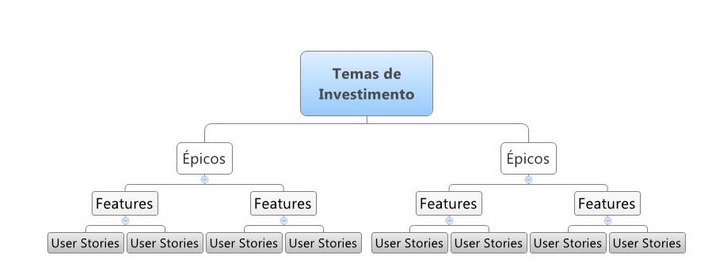
\includegraphics[scale=0.6]{rastreabilidade_vertical}
				\caption[Exemplo de Estratégia de Rastreabilidade Vertical]{Exemplificação visual da estratégia de rastreabilidade vertical.}
				\label{fig:rastreabilidade_vertical}
			\end{figure}
			\ \newline
			\subsubsection[Detalhamento dos Atributos para Rastreabilidade]{Detalhamento dos Atributos para Rastreabilidade}
			\label{subsubsec:tgr_rastreabilidade_detalhe}
				\begin{table}[h]
					\centering
					\begin{tabular}{|p{2cm}|p{7cm}|p{3cm}|}
						\hline
						\multicolumn{3}{|c|}{Atributos de Tema de Investimento} \\
						\hline
						& Valor & Descrição \\ \hline
						ID & $PT - código\_ tema\_investimento $ & Identificador do Tema de Investimento - Nível de Portfólio \\ \hline
						\hline
						\multicolumn{3}{|c|}{Atributos de Épicos} \\
						\hline
						& Valor & Descrição \\ \hline
						ID & $PT - código\_tema\_investimento\ : código\_épico $ & Identificador do Épico - Nível de Portfólio \\ \hline
						Data Início & $Data$ & Data planejada de iniciação do épico \\ \hline
						Data Encerramento & $Data$ & Data planejada para encerramento do épico \\ \hline
						\hline
						\multicolumn{3}{|c|}{Atributos de Feature} \\
						\hline
						& Valor & Descrição \\ \hline
						ID & $PR - código\_tema\_investimento : código\_épico : código\_feature$ & Identificador da Feature existente dentro de um determinado épico - Nível de Programa \\ \hline
						\hline
						\multicolumn{3}{|c|}{Atributos de User Stories} \\
						\hline
						& Valor & Descrição \\ \hline
						ID & $T - código\_tema\_investimento : código\_épico : código\_feature : código\_user\_stories$ & Identificador de um User Story existente dentro de uma determinada Feature - Nível de Time \\ \hline
					\end{tabular}
					\caption[Detalhamento dos Atributos para Rastreabilidade]{Detalhamento dos atributos para rastreabilidade, vale ressaltar que os códigos são compostos de dois dígitos. Exemplo: T:01:02:04:12.}
					\label{tab:atributo_rastreabilidade}
				\end{table}

	\ \newline
	\section[Atributos de Requisitos]{Atributos de Requisitos}
	\label{sec:tgr_atributos}
		Atributos de requisitos são conceitos que caracterizam o requisito de acordo com um dado padrão. Os atributos aos quais os requisitos serão relacionados são:
		\begin{itemize}
			\item{Prioridade;}
			\item{Estabilidade;}
			\item{Risco.}
		\end{itemize}
		\ \indent Nas subseções a seguir são apresentados a formalização do padrão desses atributos de requisitos.

		\subsection[Prioridade]{Prioridade}
		\label{subsec:tgr_atributos_prioridade}
			Este atributo é utilizado para determinar qual a importância do requisito com relação ao funcionamento ideal do sistema. As opções para este atributo são:
			\begin{itemize}
				\item{\textbf{Essencial}: Indica um requisito sem o qual o sistema não entra em funcionamento. Requisitos essenciais são requisitos imprescindíveis, que devem ser implementados impreterivelmente;}
				\item{\textbf{Importante}: Indica um requisito sem o qual o sistema entra em funcionamento, mas de forma não satisfatória. Requisitos importantes devem ser implementados, mas, se não forem, o sistema poderá ser implantado e usado mesmo assim;}
				\item{\textbf{Desejável}: Indica um requisito que não compromete as funcionalidades básicas do sistema, isto é, o sistema pode funcionar de forma satisfatória. Requisitos desejáveis são requisitos que podem ser deixados para versões posteriores do sistema, caso não haja tempo hábil para implementá-los na versão que está sendo especificada.}
			\end{itemize}

		\subsection[Estabilidade]{Estabilidade}
			Este atributo está interligado com a possibilidade do requisito sofrer modificações ao longo do projeto ou em seu tempo de vida do sistema. As opções para este atributo são:
			\begin{itemize}
				\item{\textbf{Alta}: Indica um requisito muito estável, ou seja, é pouco provável que o requisito em questão sofra mudanças no decorrer do projeto;}
				\item{\textbf{Média}: Indica um requisito que tem uma probabilidade média de sofrer alguma mudança;}
				\item{\textbf{Baixa}: Indica um requisito não estável, ou seja, é muito provável que o requisito em questão necessite de alguma mudança no futuro.}
			\end{itemize}

		\subsection[Risco]{Risco}
			Relacionado à possibilidade do requisito gerar algum risco capaz de prejudicar ou até mesmo abortar o desenvolvimento do sistema. As opções para este atributo são:
			\begin{itemize}
				\item{\textbf{Alto}: Indica que os riscos de impactos são grandes e significativos;}
				\item{\textbf{Médio}: Indica que os riscos de impactos são grandes mas com impactos não tanto significativos;}
				\item{\textbf{Baixo}: Indica a ausência de riscos de impacto no desenvolvimento do sistema.}
			\end{itemize}
			\ \indent Na Tabela \ref{tab:atributos_requisitos} é apresentado um pequeno exemplo que torna mais clara a aplicação desses atributos de requisitos às histórias de usuários desenvolvidas.

			\begin{table}[h]
				\centering
				\begin{tabular}{|c|c|c|c|}
					\hline
					Requisito & Prioridade & Estabilidade & Risco \\ \hline
					Cadastrar Exemplo & Essencial & Alta & Baixo \\ \hline
					Remover Exemplo & Importante & Média & Baixo \\ \hline
					Atualizar Exemplo & Essencial & Alta & Médio \\
					\hline
				\end{tabular}
				\caption[Exemplo de Matriz de Atributos]{Exemplo de Matriz de Atributos.}
				\label{tab:atributos_requisitos}
			\end{table}